\section{Results}
\label{sec:results_applications}

\begin{figure*}[t!]
\hskip -3mm
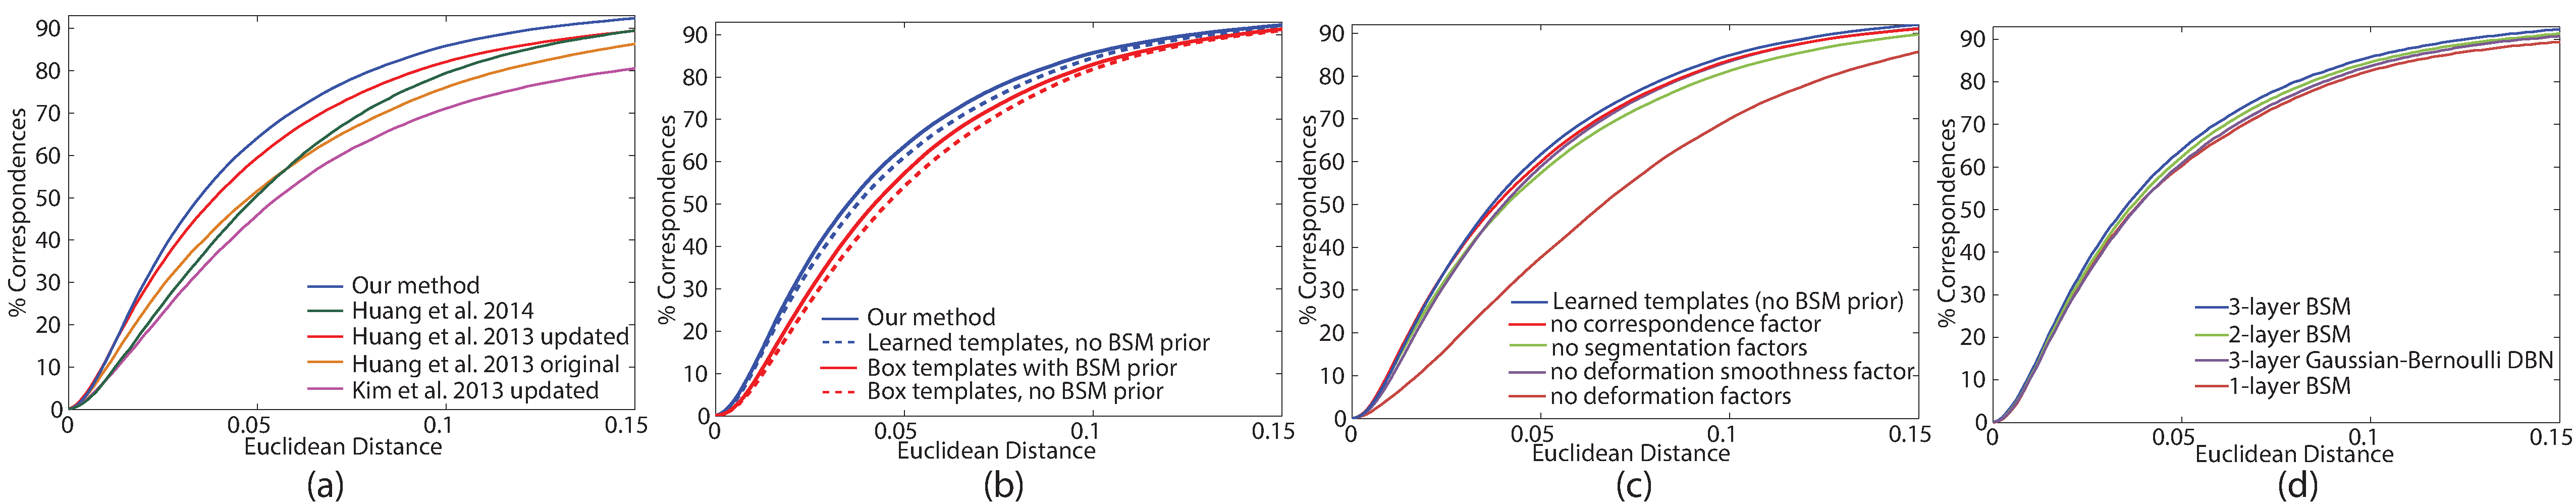
\includegraphics[width=1.03\textwidth]{figures/CORRECTED_correspondence_all.pdf}
\vskip -3mm
\caption{Correspondence accuracy of our method in Kim et al.'s benchmark versus (a) previous approaches, (b) using box templates and skipping the BSM surface prior, (c) skipping factors from the CRF deformation model, (d) versus alternative Deep Boltzmann Machine formulations.}
\vskip -8mm
\label{fig:correspondence_accuracy_all}
\end{figure*}

We now describe the experimental validation of our method for computing semantic point correspondences, shape segmentation, fine-grained classification, and synthesis.

\textbf{Correspondence accuracy.} We evaluated the performance of our method on the recent benchmark provided by Kim et al. \shortcite{Kim13}. We refer to it as BHCP benchmark. The benchmark provides positions of ground-truth points in a collection of $404$ shapes from Trimble Warehouse including bikes, helicopters, chairs and airplanes. We compared our algorithm with previous methods whose authors made their results publically available or agreed to share results with us on the same benchmark: Figure \ref{fig:correspondence_accuracy_all}a demonstrates the performance of our method, the box template fitting method by Kim et al. \shortcite{Kim13}, the local non-rigid registration method by Huang et al. \shortcite{Huang13}, and the functional map network method also by Huang et al \cite{Huang14}. We report the performance of Huang et al.'s method \shortcite{Huang13} based on the originally published results as well as the latest updated results kindly provided by the authors. Following Kim et al.'s protocol, we measure the Euclidean distance error between each provided ground-truth point position and its corresponding point position predicted by the competing methods averaged over all the pairs of shapes in the benchmark. The y-axis demonstrates the fraction of correspondences predicted correctly below a given Euclidean error threshold shown on the x-axis. We stress that all methods are compared using the same protocol evaluated over all the pairs of the shapes contained in the benchmark, as also done in previous work. The performance of our algorithm is reported using the BSM surface prior together with the CRF deformation model. Our \rev{part templates} were initialized based on the co-segmentations provided by Kim et al. (no manual segmentations were used). Our surface prior was learned in a subset of the large datasets used in Kim et al. ($1509$ airplanes, $408$ bikes, $3701$ chairs, $406$ helicopters). We did not use their whole dataset because we excluded shapes whose provided template fitting error according to their method was above the median error value for airplanes and chairs, and above the $90$th percentile for bikes and chairs indicating possible wrong rigid alignment. A few tens of models could also not be downloaded based on the provided original web links. To ensure a fair comparison, we updated the performance of Kim et al. by learning the template parameters in the same subset as ours. Their method had slightly better performance compared to using the original dataset ($0.95\%$ larger fraction of correspondences predicted correctly at distance $0.05$). Huang et al.'s reported experiments and results do not make use of the large datasets, but are based on pairwise alignments and networks within the ground-truth sets of the shapes in the benchmark. Figure \ref{fig:correspondence_accuracy_all}a indicates that our method outperforms the other algorithms. In particular, we note that even if we initialized our method with Kim et al.'s segmentations, the final output of our method is significantly better: $18.2\%$ more correct predictions at $0.05$ distance than Kim et al.'s method. 

We provide images of the corresponding feature points and labeled segmentations for the shapes of our large datasets in the supplementary material as well as Figures \ref{fig:teaser} (left) and \ref{fig:chairs_synthesis} (left). All these results were produced by initializing our method with the co-segmentations provided by Kim et al. (no manual shape segmentation was used). We also provide correspondence accuracy plots for each category separately in the supplementary material. 



%\begin{figure}[t!]
%\centering
%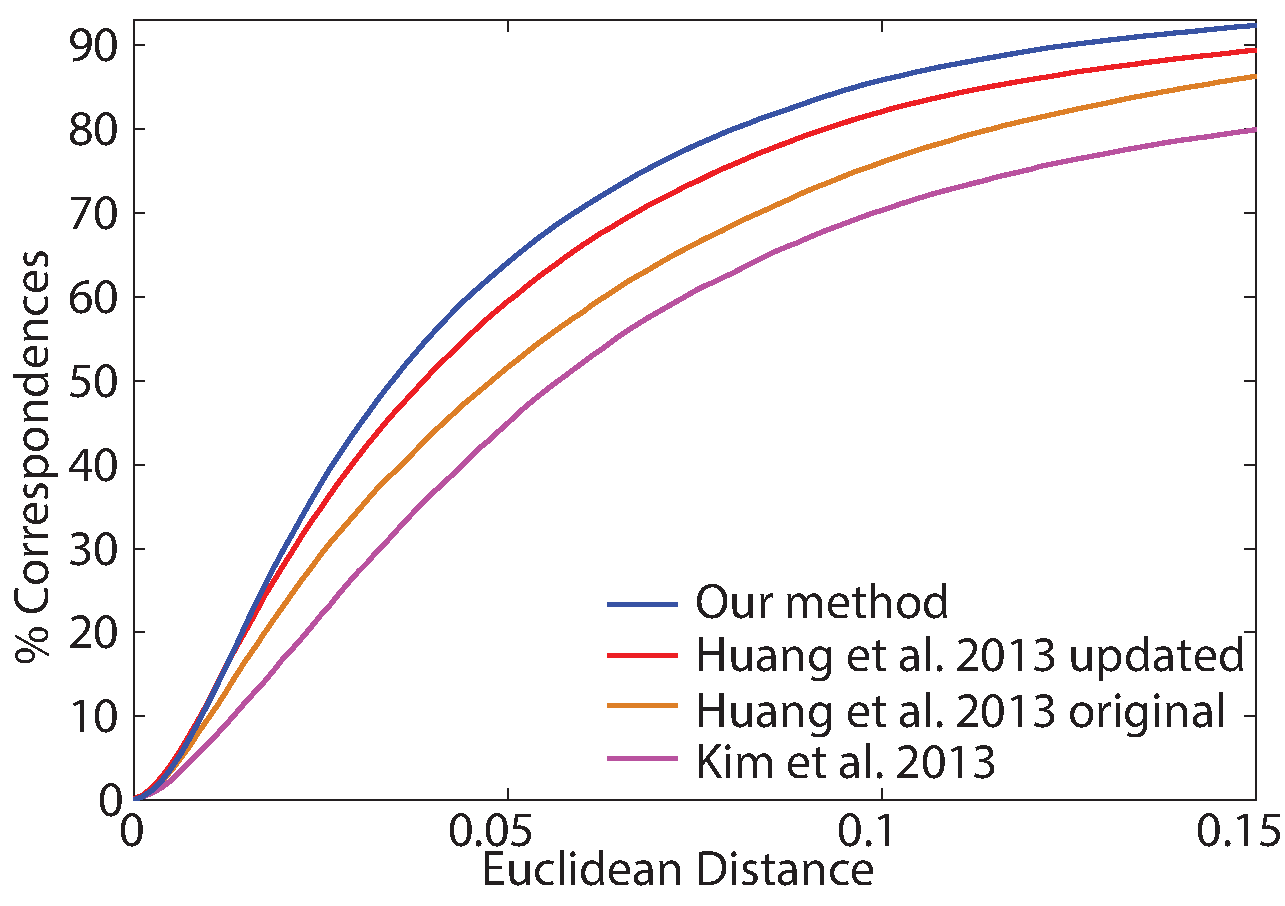
\includegraphics[width=.9\columnwidth]{figures/CORRECTED_correspondence_average.pdf}
%\caption{Correspondence accuracy of our method in Kim et al.'s benchmark compared to previous approaches.}
%\label{fig:correspondence_accuracy_main}
%\end{figure}

\textbf{Alternative formulations.} We now evaluate the performance of our method compared to alternative formulations. First, we show the performance of our method in the case it does not learn \rev{part templates}, but instead uses the same mean-field deformation procedure on the box templates provided by Kim et al. In other words, we deform boxes instead of learned parts. Figure \ref{fig:correspondence_accuracy_all}b shows that the correspondence accuracy is significantly better with the learned \rev{part templates}. In the same plot, we show the performance of the two versions of our method with and without the BSM surface prior. We note that using the BSM prior improves correspondence accuracy either in the case of box or learned part templates. 

%Figure \ref{mf_iterations} demonstrates the improvement in the correspondence accuracy for each mean-field iteration for learning the \rev{part templates}. After about $8$ iterations, mean-field converges, and there is no more significant improvement. 

%\begin{figure}[t]
%\centering
%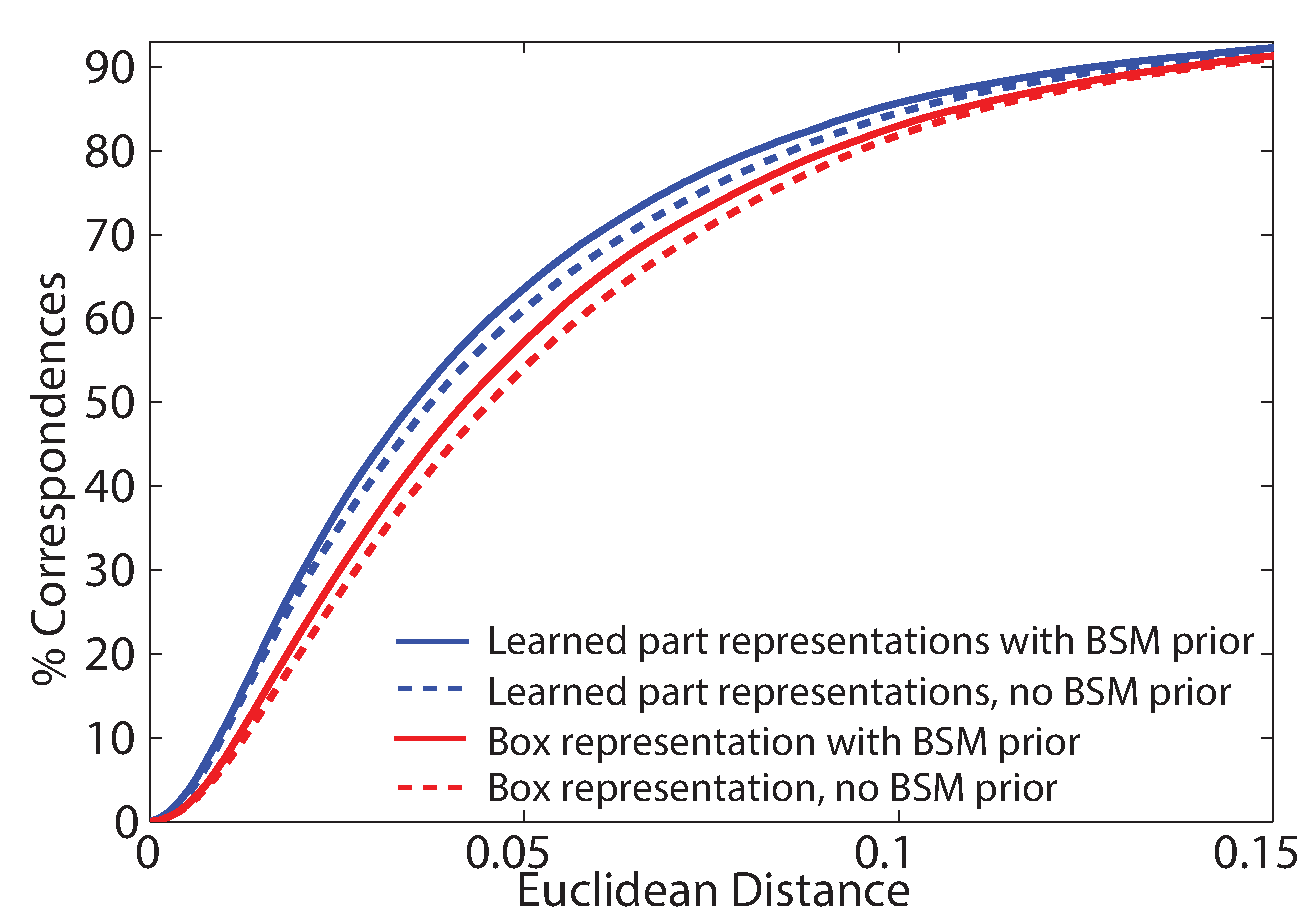
\includegraphics[width=.9\columnwidth]{figures/CORRECTED_correspondence_accuracy_different_models.pdf}
%\caption{Correspondence accuracy of our method in Kim et al.'s benchmark versus using deformed box representations or skipping the BSM surface prior.}
%\label{fig:correspondence_accuracy2}
%\end{figure}

%\begin{figure}[t]
%\centering 
%\includegraphics[width=1.0\columnwidth]{figures/accuracy_learned}
%\caption{ Fraction of correspondences predicted correctly below $0.05$ error threshold versus running more mean-field %iterations for learning the \rev{part templates} (variables $\bY$).  }
%\label{fig:mf_iterations}
%\end{figure}
 
We also evaluate the performance of our method by testing the contribution of the different factors used in the CRF deformation model. Figure \ref{fig:correspondence_accuracy_all}c shows the correspondence accuracy in the same benchmark by using all factors in our model (top curve), without using the unary deformation, deformation smoothness, correspondence or segmentation factors. For all these alternative models, we do not include the BSM prior to factor out its influence. As shown in the plot, all factors contribute to the improvement of the performance. In particular, skipping the deformation or segmentation parts of the model cause a noticeable performance drop. 

Finally, we evaluate the performance of our method by using different formulations of the surface prior. Figure \ref{fig:correspondence_accuracy_all}d demonstrates the correspondence accuracy of our three-layer BSM model (original model), versus a two-layer and a single-layer BSM model. In addition, we include a comparison with a Deep Boltzmann Machine that uses Gaussian instead of Beta distributions (Gaussian-Bernoulli DBM) using three layers and the same training procedure. Our three-layer BSM model provides the best performance. Using more layers did not yield any significant improvement based on our datasets.

%\begin{figure}[t]
%\centering
%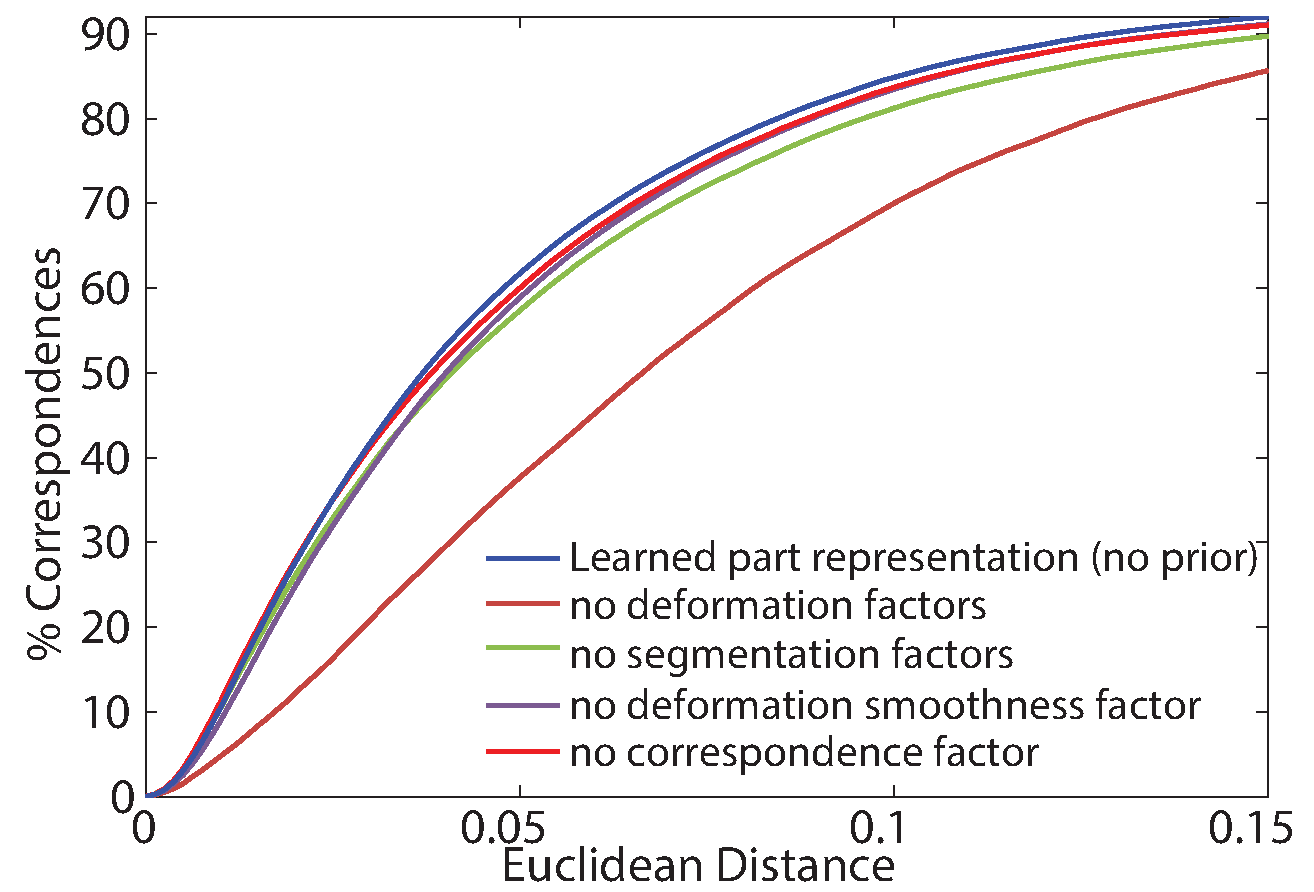
\includegraphics[width=.9\columnwidth]{figures/CORRECTED_correspondence_factor_diff.pdf}
%\caption{Correspondence accuracy of our method in Kim et al.'s benchmark versus skipping different factors from the CRF model.}
%\label{fig:correspondence_accuracy3}
%\end{figure}

\vskip -2mm
\begin{table}[h]
\centering
\begin{tabular}{|@{}c@{}|@{}c@{}|@{}c@{}|@{}c@{}|@{}c@{}|}
\hline
 Category           & Num.            & \,Kim et al.\, & Our          & Num. \\
 (Dataset)          & \,shapes\,      & \,(our init.)\,  & \,method\, & \,groups\, \\  
\hline  
 Bikes (BHCP)        & 100   & 76.8 & 82.3 & 2 \\
 Chairs (BHCP)       & 100   & 81.2 & 86.8 & 2\\
 Helicopters (BHCP)  & 100   & 80.1 & 87.4 & 1 \\
 Planes (BHCP)       & 104   & 85.8 & 89.6 & 2 \\
\hline  
 Lamps (COSEG)      & 20    & 95.2 & 96.5 & 1 \\
 Chairs (COSEG)     & 20    & 96.7 & 98.5& 1 \\
 Vase (COSEG)       & 28    & 81.3 & 83.3& 2 \\
 Quadrupeds (COSEG) & 20    & 86.9 & 87.9& 3 \\
 Guitars (COSEG)    & 44    & 88.5 & 89.2 & 1 \\
 Goblets (COSEG)    & 12    & 97.6 & 98.2 & 1\\
 Candelabra (COSEG) & 20    & 82.4 & 87.8 & 3\\
 Large Chairs (COSEG) & 400 & 91.2 & 92.0 & 5 \\
 Large Vases (COSEG)  & 300 & 85.6 & 83.0 & 5 \\
\hline 
\end{tabular}
\vskip -1mm
\caption{Labeling accuracy of our method versus Kim et al.}
\label{table:results_coseg}
\vskip -2mm
\end{table}

\begin{figure*}[t]
\centering
\includegraphics[width=0.95\textwidth]{figures/teaser_chair}
\vskip -2mm
\caption{Left: Shape correspondences and segmentations for chairs. Right: Synthesis of new chairs}
\label{fig:chairs_synthesis}
\vskip -8mm
\end{figure*}

\textbf{Segmentation accuracy.} We now report the performance of our method for shape segmentation. We evaluated the segmentation performance on the COSEG dataset \cite{Wang12} and a new dataset we created: we labeled the parts of the $404$ shapes used in the BHCP correspondences benchmark. We provide images of the ground-truth segmentations in the supplementary material. We compared our method with Kim et al.'s segmentations in these datasets based on the publically available code and data. These are the same segmentations that we used to initialize our method (no manual segmentations were used). For both methods, we evaluate the labeling accuracy by measuring the fraction of faces for which the part label predicted by our method agrees with the ground-truth label. Since our method provides segmentation at a point cloud level, we transfer the part labels from points to faces using the same graph cuts as in Kim et al. Table \ref{table:results_coseg} shows that our method yields better labeling performance. The difference is noticeable in complex shapes, such as helicopters, airplanes, bikes and candelabra.  The same table reports the number of clusters (groups) used in our model. We note that our method could be initialized with any other unsupervised technique. This table indicates that our method tends to improve the segmentations it was initialized with. 

\textbf{Fine-grained classification.} \rev{The uppermost layer of the BSM model can be used to produce a compact, class-specific shape descriptor. We demonstrate its use in the context of fine-grained classification. For this purpose, we labeled the BHCP benchmark shapes with fine-grained class labels: we categorized airplanes into commercial jets, fighter jets, propeller aircraft and UAVs, chairs into benches, armchairs, side and swivel chairs, and bikes into bicycles, tricycles and motorbikes. We compute activation probabilities in the uppermost layer through mean-field inference given each input shape, and used those as  descriptors. Using $10$ training examples per class, and a single nearest neighbor classification scheme based on $L^1$ norm distance, the rest of the shapes were classified with accuracy $92\%$, $94\%$, $96.5\%$ for airplanes, chairs, and bikes respectively. Descriptors, results, training and test splits are included in the supplementary material.}

\textbf{Shape synthesis.} Figure \ref{fig:teaser}(right) and \ref{fig:chairs_synthesis}(right) demonstrates synthesized chairs and airplanes using samples from the BSM model trained on these large collections. Our shape synthesis procedure makes use of the shape parts segmented by our method in these collections. However, not all shapes are segmented perfectly: even if the labeling accuracy of our method is high as demonstrated above, minor errors along segmentation boundaries (e.g., mislabeled individual faces crossing boundaries) cause visual artifacts when shapes are assembled from these segmented parts. Such errors are common in graph cuts. Corrections would require re-meshing or other low-level mesh operations. We instead manually flagged $25\%$ of airplanes and $40\%$ of chairs with imperfect segmentation boundaries. These were excluded during the nearest neighbors procedure for selecting parts given the BSM samples. We still believe that the amount of human supervision for this process is much smaller compared to previous generative models \cite{Kalogerakis12} that required manually specified shape segmentations for at least half or the whole input collections. We also conducted a perceptual evaluation of our synthesized shapes with $31$ volunteers recruited through Amazon Mechanical Turk. Our user study indicates that the shapes produced by our model were seen as plausible as the training shapes of the input collections. We include the user study details and results in the supplementary material. We also provide images of $500$ synthesized airplanes and chairs in the supplementary material.   

\textbf{Running times.} The mean-field procedure (Algorithm \ref{algorithm}) requires $6$ hours for our largest dataset (3K chairs). Learning the BSM model requires $45$ hours on the same dataset. Running times are reported on a E5-2697 v2 processor. Running times scale linearly with the dataset size.

\vspace{-2mm}



%%%% OLD TABLE
%\begin{table}[h]
%\hskip -3mm
%\footnotesize
%\begin{tabular}{|@{}c@{}|@{}c@{}|@{}c@{}|@{}c@{}|@{}c@{}|@{}c@{}|}
%\hline
% Category & Num.       & \cite{Huang14}\,   & \cite{Kim13}\, & Our          & Num. \\
% (Dataset)& \,shapes\, & \,(F-maps)\,       & \,(our init.)\,  & \,method\, & \,groups\, \\  
%\hline  
% Bikes (BHCP)         & 100   & N/A           & 76.8 & \textbf{82.3} & 2 \\
% Chairs (BHCP)        & 100   & N/A           & 81.2 & \textbf{86.8} & 2 \\
% Helicopters (BHCP)   & 100   & N/A           & 80.1 & \textbf{87.4} & 1 \\
% Planes (BHCP)        & 104   & N/A           & 85.8 & \textbf{89.6} & 2 \\
%\hline  
% Lamps (COSEG)        & 20    & 96.1          & 95.2 & \textbf{96.5} & 1 \\
% Chairs (COSEG)       & 20    & 93.9          & 96.7 & \textbf{98.5} & 1 \\
% Vase (COSEG)         & 28    & \textbf{88.5} & 81.3 & 83.3          & 2 \\
% Quadrupeds (COSEG)   & 20    & 74.8          & 86.9 & \textbf{87.9} & 3 \\
% Guitars (COSEG)      & 44    & \textbf{93.4} & 88.5 & 89.2          & 1 \\
% Goblets (COSEG)      & 12    & 91.2          & 97.6 & \textbf{98.2} & 1 \\
% Candelabra (COSEG)   & 20    & \textbf{93.1} & 82.4 & 87.8          & 3 \\
% Large Chairs (COSEG) & 400   & \textbf{98.1} & 91.2 & 92.0          & 5 \\
% Large Vases (COSEG)  & 300   & \textbf{94.3} & 85.6 & 83.0          & 5 \\
%\hline 
%\end{tabular}
%\vskip -2mm
%\caption{Labeling accuracy of our method versus Kim et al.}
%\label{table:results_coseg}
%\vskip -2mm
%\end{table}


